\documentclass{article}
\usepackage{graphicx} % \includegraphics
\usepackage{hyperref} % \href
\usepackage{subcaption}
\usepackage{listings}
\usepackage{xcolor}
\usepackage{booktabs}

\lstset{
    language=Python,
    basicstyle=\ttfamily\footnotesize,
    keywordstyle=\color{blue},
    stringstyle=\color{green},
    commentstyle=\color{gray},
    showstringspaces=false,
    numbers=left,
    numberstyle=\tiny,
    frame=single
}

\graphicspath{{./img/}}

\begin{document}
\title{
\includegraphics[scale=.2]{img/logo-unipi/logo.png} \\[3ex] A.S.E - 2024/2025 \\ Final Delivery}
\author{{\large \emph{EzGacha Team}} \\[1ex] Gioele Dimilta \\ Andrea Mugnai \\ Jacopo Tucci}
\date{}

\pagenumbering{gobble}
\maketitle

\newpage
\pagenumbering{arabic}
\tableofcontents
\newpage
\section{Gachas overview}
Gachas are a popular type of random reward system often used in video games and other digital media. They typically involve spending in-game currency or real money to obtain random items, characters, or other rewards.
We have chosen pixel art images for the gacha (figure \ref{fig:gachas_images}).
\begin{figure}[h!]
    \centering
    \begin{subfigure}[b]{0.3\textwidth}
        \centering
        
\includegraphics[width=\textwidth]{img/gacha/Cyclops (non-common).jpg}
        \caption{Cyclops}
        \label{fig:cyclops}
    \end{subfigure}
    \hfill
    \begin{subfigure}[b]{0.3\textwidth}
        \centering
        
\includegraphics[width=\textwidth]{img/gacha/Dragon (epic).jpg}
        \caption{Dragon}
        \label{fig:dragon}
    \end{subfigure}
    \hfill
    \begin{subfigure}[b]{0.3\textwidth}
        \centering
        
\includegraphics[width=\textwidth]{img/gacha/Phoenix (legendary).jpg}
        \caption{Phoenix}
        \label{fig:phoenix}
    \end{subfigure}
    \vspace{1em} 
    \begin{subfigure}[b]{0.3\textwidth}
        \centering
        
\includegraphics[width=\textwidth]{img/gacha/Kraken (legendary).jpg}
        \caption{Kraken}
        \label{fig:kraken}
    \end{subfigure}
    \hfill
    \begin{subfigure}[b]{0.3\textwidth}
        \centering
        
\includegraphics[width=\textwidth]{img/gacha/Minotaur (epic).jpg}
        \caption{Minotaur}
        \label{fig:minotaur}
    \end{subfigure}
    \hfill
    \begin{subfigure}[b]{0.3\textwidth}
        \centering
        
\includegraphics[width=\textwidth]{img/gacha/Vampire (epic).jpg}
        \caption{Vampire}
        \label{fig:vampire}
    \end{subfigure}
    \caption{Gachas Images}
    \label{fig:gachas_images}
    \label{fig:gachas_images}
\end{figure}

Each of our gachas includes a description that details the mythological creature represented.

\subsection{Rarities}
Gachas often come in different rarities, which determine the likelihood of obtaining certain items. Our rarities are defined according to the following probabilities (table \ref{tab:rarity}).

\begin{table}[ht!] 
    \centering
    \begin{tabular}{|c|c|c|c|c|}
        \hline
        \textbf{Common} & \textbf{Uncommon} & \textbf{Rare} & \textbf{Epic} & \textbf{Legendary} \\
        \hline
        $50\%$          & $30\%$            & $10\%$        & $8\%$         & $2\%$              \\
        \hline
    \end{tabular}
\caption{Rarity probabilities}
\label{tab:rarity}
\end{table}

\newpage
\section{Architecture}
The architecture follows a microservices-based approach, with each service dedicated to a specific functionality. The overall structure is depicted in Figure \ref{fig:microfreshener_architecture}, generated using the microFreshener tool to model microservice architectures, identify architectural smells, and propose refactoring solutions.
\begin{figure}[ht]
    \centering
    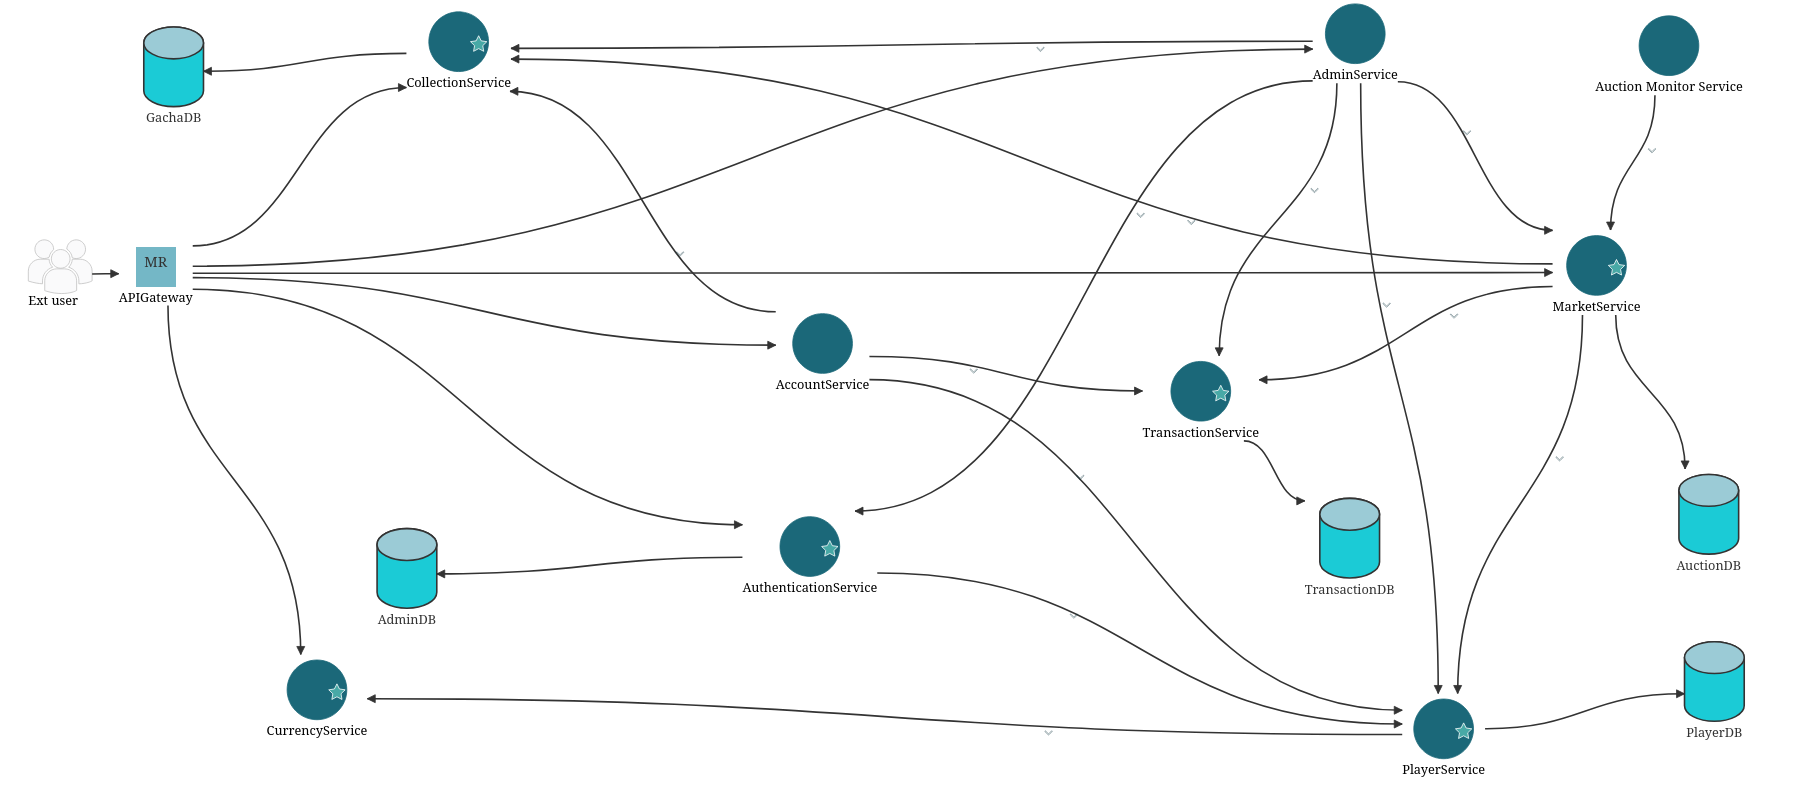
\includegraphics[width=12cm]{img/microfreshener/microFreshenerArchitecture.png}
    \caption{MicroFreshener architecture}
    \label{fig:microfreshener_architecture}
\end{figure}

In our case, the \emph{circuit breaker} design pattern was implemented to mitigate the \emph{wobbly service interaction smell}, and no further architectural smells were identified during the analysis phase.
\newline
In the following sections, the functionalities of the microservices within our system will be briefly described, along with their interactions, as illustrated in figure \ref{fig:microfreshener_architecture} and \ref{fig:general_architecture}.

\subsection{Microservice Overview}
\begin{itemize}
    \item \textbf{Authentication} microservice handles user authentication, \emph{JWT token} issuance, and logout. It acts as an OAuth 2-compliant authorization server, authenticating clients, validating user credentials, and issuing access tokens.
    \item \textbf{Account} microservice manages user account operations, including user creation, updates, deletion, and retrieval of player-specific data such as collections, wallet currency, and transactions.
    \item \textbf{Admin} microservice provides a suite of administrative functionalities. It includes features for user and collection management, marketplace auction handling, and transaction processing.
    \item \textbf{Gacha} microservice provides a comprehensive range of functionalities for managing \emph{gacha} item collections, including retrieval, updating, addition, and deletion. It also incorporates a random item rolling mechanism based on rarity, enabling interaction with a marketplace-like feature.
    \item \textbf{Market} microservice provides functionalities for managing auctions and transactions related to \emph{gacha} items. It enables the creation of auctions, placing bids, managing payments, and closing auctions. Payment processing is managed using \emph{Celery} for asynchronous task execution.
    \item \textbf{Celery} microservice is responsible for managing asynchronous background tasks related to payment processing.
    \item \textbf{Player} microservice manages player-related data, including operations like retrieving, modifying, and deleting player information.
    \item \textbf{Currency} microservice is designed to manage player currency transactions, enabling players to make purchases using in-game currency.
    \item \textbf{Transaction} microservice handles transactions related to market auctions. It provides endpoints to create new transactions, retrieve transactions by user or UUID, and view transactions from both buyer and seller perspectives.
    \item \textbf{RabbitMQ} microservice manages task queuing for \emph{Celery} Workers sends tasks to workers for auction closing operations and supports task rescheduling if worker fails; we use RabbitMQ message broker technology Dockerized with \emph{rabbitmq: 3-management} image.
\end{itemize}

\begin{figure}[ht]
    \centering
    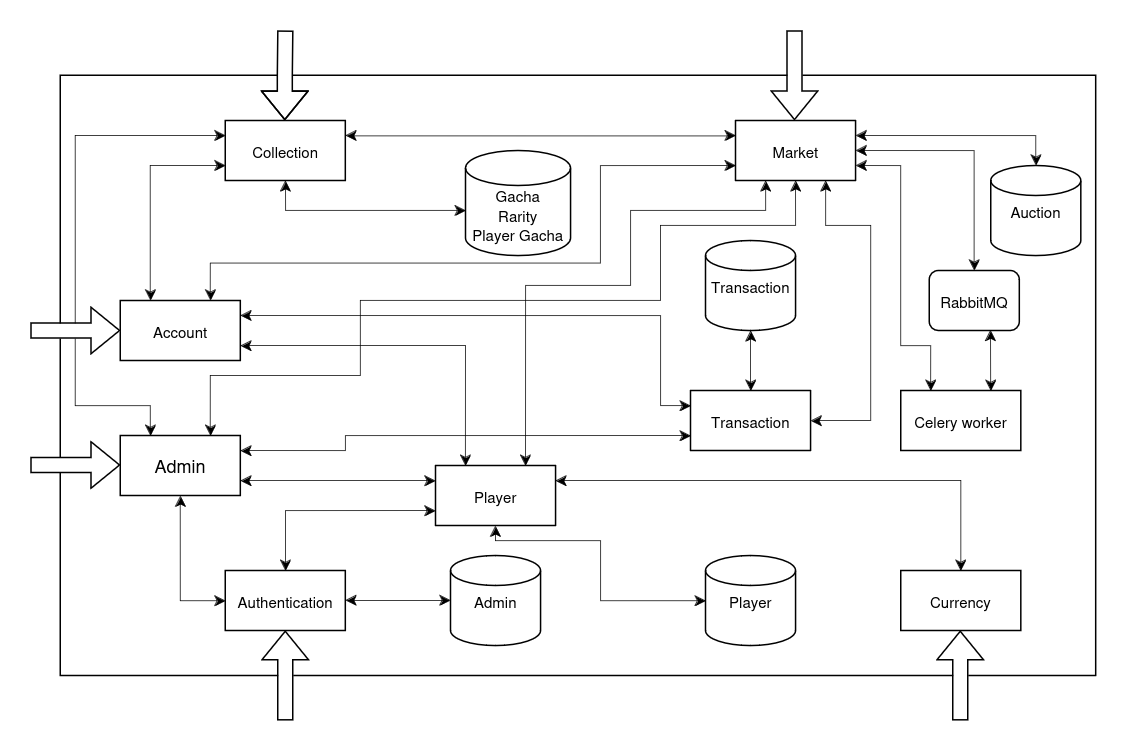
\includegraphics[width=12cm]{img/architecture/architecture-v2.drawio.png}
    \caption{General architecture}
    \label{fig:general_architecture}
\end{figure}

\subsection{Service Interconnections}
\begin{itemize}
    \item \textbf{Authentication}
        \begin{itemize}
            \textbf{Player}: \emph{Authentication} is connected with \emph{Player Service} because it needs to retrieve player information, including the password hash, to verify user credentials during the login process. 
        \end{itemize}
    \item \textbf{Account}
        \begin{itemize}
            \item \textbf{Player}: The \emph{Account service} is connected to the \emph{Player Service} because it needs to manage player data, including the creation, deletion, and modification of player information. This connection is essential to ensure that all player-related operations are centralized and consistent.
            \item \textbf{Gacha}: The \emph{Account Service} is connected with \emph{Gacha Service} because it needs to retrieve a player's collection of items. This collection can include various items that the player has acquired through different activities within the system. The connection with \emph{Gacha Service} allows to display and manage the player's collection, providing a comprehensive overview of the items owned by the player.
            \item \textbf{Transaction}: The \emph{Account Service} is connected to the \emph{Transaction Service} because it needs to retrieve all transactions and specific transaction details for a player. This connection is crucial for tracking the player's financial activities, such as purchases, sales, and other transactions. The connection is essential for features such as viewing the player's transaction history.
            \item \textbf{Market}: The \emph{Account Service} is connected to \emph{Market Service} because it needs to check for active auctions before allowing a player to delete their account. This check is important to ensure that no ongoing auctions are disrupted due to the deletion of the player's account. If a player has active auctions, \emph{Account Service} must prevent account deletion until all auctions are concluded.
        \end{itemize} 
    \item \textbf{Admin}
        \begin{itemize}
            \item \textbf{Authentication}: The \emph{Admin Service} is connected to \emph{Authentication Service} because it needs to authenticate admin users. This connection ensures that only authorized admin users can access the administrative functionalities provided by \emph{Admin service}.
            \item \textbf{Player}: The \emph{Admin Service} is connected to \emph{Player Service} because it needs to manage player data, including: retrieving all players, getting specific player information, modifying player details, and deleting players.
            \item \textbf{Gacha}: The \emph{Admin service} is connected to \emph{Gacha Service} because it needs to manage the collection of gacha items. This includes adding new gacha items, modifying existing gacha items, removing gacha items, and retrieving a player's collection.
            \item \textbf{Market}: The \emph{Admin Service} is connected to \emph{Market Service} because it needs to manage auctions. Including retrieving all auctions (open and closed), getting specific auction details, closing auctions, and processing payments for auctions.
            \item \textbf{Transaction}: The \emph{Admin Service} is connected to \emph{Transaction Service} because it needs to retrieve all transactions for a specific player, allowing to perform administrative tasks.
        \end{itemize} 
    \item \textbf{Market}
        \begin{itemize}
            \item \textbf{Gacha}: The \emph{Market Service} is connected to \emph{Gacha Service} because it needs to retrieve information about gacha items. This includes getting all gacha items and specific gacha item details. This connection is essential for displaying gacha items in auctions and ensuring that the marketplace has accurate  up-to-date information about the items being auctioned.
            \item \textbf{Player}: The \emph{Market Service} is connected to \emph{Player Service} because it needs to retrieve player information. Including player details and  collection. Allowing  \emph{Market service} to verify the ownership of gacha items, retrieve player wallet information, and update player collections and wallets after transactions.
            \item \textbf{Transaction}: The \emph{Market Service} is connected to \emph{Transaction Service} because it needs to create and manage transactions related to auctions. This includes recording bids, processing payments, and updating transaction records. The connection ensures that all financial transactions within the marketplace are accurately recorded and managed.
        \end{itemize}
    \item \textbf{Gacha}
    \begin{itemize}
        \item \textbf{Player}: The \emph{Gacha Service} is connected to \emph{Player Service} because it needs to update the player's wallet when a player performs a roll. This interaction ensures that the player's wallet is deducted the appropriate amount for the roll action.
    \end{itemize}
    \item \textbf{Transaction}
    \begin{itemize}
        \item The \emph{Transaction Service} is connected to \emph{Market Service} because it needs to retrieve auction details related to transactions. This includes getting specific auction details by UUID and retrieving all auctions associated with a player. This connection is crucial for ensuring that transaction records are accurate and up-to-date.
    \end{itemize}
    \item \textbf{Currency}
    \begin{itemize}
        \item \textbf{Player}: The \emph{Currency Service} is connected to \emph{Player Service} because it needs to update the player's wallet when a player purchases the in game-currency. This interaction ensures that the player's wallet is credited with the purchased amount, maintaining the financial integrity of the player's account within the system.
    \end{itemize}
    \item \textbf{RabbitMQ}
    \begin{itemize}
        \item \textbf{Market}: \emph{RabbitMQ} is connected to \emph{Market Service} because it needs to handle asynchronous tasks related to auctions. This connection ensures that tasks such as closing auctions and processing payments are executed asynchronously, allowing \emph{Market service} to handle other requests without waiting for these tasks to complete.
\item \textbf{Celery}: \emph{RabbitMQ} is connected to \emph{Celery worker} because it needs to manage and distribute asynchronous tasks. This connection allows the \emph{Celery worker} to receive tasks from \emph{RabbitMQ} and execute them. For instance, when a task to close an auction is scheduled, \emph{RabbitMQ} sends this task to the \emph{Celery worker}, which then performs the necessary actions to close an auction and process any associated payments.
    \end{itemize}
\end{itemize}

\newpage

\section{User Stories}
In the following section, we describe \emph{User Stories} for the player, specifying the endpoints and the microservices involved in realizing each story.\\ We use the index from the shared file to indicate \emph{User Stories}.
\vspace{1em}

\begin{itemize}
    \item 1) /user (Gateway, Account, Player, player\_db)
    \item 2) /user (Gateway, Account, Market, market\_db, Player, player\_db)
    \item 3) /user (Gateway, Account, Player, player\_db)
    \item 4) /login (Gateway, Authentication, Player, player\_db)
    \item 6) /user/collection (Gateway, Account, Gacha, gacha\_db)
    \item 7) /user/collection (Gateway, Account, Gacha, gacha\_db)
    \item 8) /collection (Gateway, Gacha, gacha\_db)
    \item 9) /collection/{gacha\_uuid} (Gateway, Gacha, gacha\_db)
    \item 10) /roll (Gateway, Gacha, gacha\_db, Player, player\_db, gacha\_db)
    \item 11) /currency/buy (Gateway, Currency, Player, player\_db)
    \item 13) /market (Gateway, Market, market\_db, Gacha, gacha\_db, player, Player\_db)
    \item 14) /market (Gateway, Market, Gacha, gacha\_db, market\_db)
    \item 15) /market/{auction\_uuid}/bid (Gateway, Market, market\_db)
    \item 16) /user/transactions (Gateway, Transaction, transaction\_db, Market, market\_db, Gacha, gacha\_db, Player, player\_db, Market, market\_db, transaction\_db, Market, market\_db, Gacha, gacha\_db, Player, player\_db)
    \item 17) /market/{auction\_uuid}/payment (Gateway, Market, market\_db, Player, player\_db, Transaction, transaction\_db, Player, player\_db, Gacha, gacha\_db, market\_db)
    \item 18) /market/{auction\_uuid}/payment (Gateway, Market, market\_db, Player, player\_db, Transaction, transaction\_db, Player, player\_db, Gacha, gacha\_db, market\_db)
    \item 19) *
\end{itemize}

* For \emph{User Story} index 19, which involves receiving in-game currency back when a player loses an auction, we have implemented an alternative method to address potential issues as described in Section \ref{sec:market_rules}.

\newpage

\section{Market rules} \label{sec:market_rules}
In designing the market system for our game, we have implemented some \emph{key rules and mechanisms} to ensure fair and efficient auction processes. The principal decisions and rules governing the market are as follows:
\begin{enumerate}
    \item \textbf{Bid Placement}: A player can place a \emph{bid} even \emph{without} sufficient currency. Obviously the \emph{bid} must be higher than the current highest \emph{bid} and the base price of the auction. If a player is unable to pay, for instance due to insufficient funds, the \emph{runner-up} player will become the winner.
    \item \textbf{Auction Closure}: The payment operation is automatically processed by the system at the end of the auction, therefore the amount of money offered is not actually deducted until the auction closes.
    \item \textbf{Bid Timing}: If a player places a bid in the last second of the auction, the auction timer is not extended, so if a bid is placed after the auction has closed, it will not be accepted as valid.
    \item \textbf{Auction Participation}: A player can bid on an auction even if they are the current highest bidder. They \emph{can manually close} auctions only if they are the owner, but not if the auction has active bids. \\
An \emph{Admin}, however, can close any auction, regardless of ownership or active bids, and has the authority to force payment.
    \item \textbf{Auction Creation}: Players can create auctions for \emph{gachas} they own. The system checks the player's collection to ensure they have the gacha in sufficient quantity before allowing the auction to be created. The starting price for an auction must be positive and set by the player creating the auction.
    \item \textbf{Auction Visibility}: Players can see only \emph{open} auctions. Admin have access to both open and closed auctions. Both can view detailed information about each auction, including the current highest bid, the base price, and the expiration time.
    \item \textbf{Payment and Wallet Updates}: Upon successful expired of an auction, the system \emph{updates the wallets} of both the buyer and the seller. The buyer's wallet is debited by the bid amount, and the seller's wallet is credited with the same amount. The \emph{gacha} then is automatically transferred from the seller's collection to the buyer's collection.
\end{enumerate}

\newpage

\section{Testing} \label{sec:testing_approach}
As requested our testing strategy encompassed three distinct levels of testing to ensure the robustness, reliability, and performance of our microservices architecture:

\subsection{Isolation Testing}
We conducted extensive isolation tests for each microservice, implementing a strategy that decouples the service from external dependencies:
\begin{itemize}
    \item \textbf{Mock Connectors:} We developed dedicated mock classes for database and HTTP connectors that simulate real-world interactions without external service calls.
    \item \textbf{In-Memory Data Management:} Test data is maintained entirely in memory, allowing for focused testing of service-specific functionality.
    \item \textbf{Authentication Service Example:} During login tests, the authentication service retrieves player and admin credentials from mock connector classes (\texttt{connector\_http\_mock} and \texttt{connector\_db\_mock}) instead of making actual database or external service requests.
\end{itemize}

The primary objective of isolation testing was to verify the internal logic and behavior of individual microservices independently of external systems.

\subsection{Integration Testing}
Integration tests validated the end-to-end functionality of our microservices architecture:
\begin{itemize}
    \item \textbf{Endpoint Verification:} All API endpoints were tested using HTTPS requests through the local proxy (\texttt{https://localhost}).
    \item \textbf{Real-World Simulation:} Tests utilized actual HTTPS communication protocols and genuine database interactions.
    \item \textbf{Tools:} Postman was employed to facilitate comprehensive integration testing across different service endpoints.
\end{itemize}
These tests ensured uninterrupted communication and data flow between various microservices and their respective databases.

\subsection{Performance Testing}
Performance assessments focused on evaluating system resilience and load handling:
\begin{itemize}
    \item \textbf{Concurrent Request Handling:} Extensive testing of player and admin endpoints to identify potential bottlenecks under high concurrency.
    \item \textbf{Load Simulation:} Utilized Locust for generating multiple simultaneous requests to stress-test service capabilities.
    \item \textbf{Gacha Probability Validation:} Implemented statistical analysis to verify the adherence to predefined rarity distribution in gacha mechanisms.
\end{itemize}
Performance testing was crucial in ensuring system stability and maintaining the integrity of probabilistic game mechanics.

\subsection{Testing Tools and Approach}
\begin{itemize}
    \item \textbf{Isolation \& Integration Testing:} Postman.
    \item \textbf{Performance Testing:} Locust.
    \item \textbf{Mock Frameworks:} Custom-developed mock connectors for database and HTTP interactions.
\end{itemize}
\newpage

\section{Security – Data}
In this section, we outline the security measures implemented to protect sensitive data within our system. We focus on input sanitization to prevent malicious data from entering our system and data encryption to safeguard sensitive information at rest.

\subsection{Input Sanitization Example}
In our system \emph{player\_uuid} parameter is a critical input that represents the unique identifier for a player. This input is used by the Player Service to retrieve, update, or delete player information. 
The object that use and are involved in the utilization of this variable are Player Service, that handles all operations related to player data and Player ConnectorDB, that interacts with player\_db to perform CRUD operations on this data. \\ \\
To ensure the security and integrity of the data, the \emph{player\_uuid} input is sanitized using a regular expression (UUID\_REGEX), this validates that the \emph{player\_uuid} conforms to the standard UUID format. The sanitization process involves the following steps as we can see in listing \ref{lst:check_uuid}:
\begin{itemize}
    \item \textbf{Validation}: The \emph{check\_uuid} function is used to validate the \emph{player\_uuid} input against the UUID\_REGEX pattern. This function returns the name of the invalid parameter if the input does not match the expected format.
    \item \textbf{Error Handling}:  If the \emph{player\_uuid} is invalid, an appropriate error message is returned to the client, indicating the specific parameter that failed validation.
    \item \textbf{Database Interaction}: Once the \emph{player\_uuid} is validated, it is used to interact with the database through the Player ConnectorDB. This ensures that only valid UUIDs are processed, preventing potential SQL injection attacks and ensuring data integrity.
\end{itemize}

\begin{lstlisting}[language=Python, caption={Sanitization example}, label={lst:check_uuid}]
def check_uuid(**kwargs):
    res = {'name': None}
    p = re.compile(PlayerService.UUID_REGEX, re.IGNORECASE)

    for key, value in kwargs.items():
        if p.match(value) is None:
            res['name'] = key
            break

    return res
\end{lstlisting}

\newpage

\subsection{Data Encryption}
\begin{itemize}
    \item \textbf{Encrypted Data}: Passwords are hashed using the \emph{bcrypt} library to ensure that they are stored securely. The \emph{bcrypt} library automatically generates a unique salt for each password, which is then used to hash the password itself. This ensures that even if two users have the same password, their hashed values will be different, enhancing security. uring authentication, the stored password hash is compared with the hashed input password to verify the user's identity.
    \item \textbf{Database Storage}: To ensure the security of our databases, we utilize a Docker image that enforces both SSL connections and encryption at rest. This setup is applied to all our databases, including AdminDB, GachaDB, MarketDB, PlayerDB, and TransactionDB. Each database has its own server certificate (\emph{server.crt}) and server key (\emph{server.key}). \\
    The Dockerfile in each db is configured to initialize the database with SSL support and encryption. Here is an overview of the key components:
    \begin{enumerate}
        \item Base Image: cybertecpostgresql/postgresql-ee-demo:16
        \item Certificate and Key generation: The initialization script (\emph{ssl\_init.sh}) ensures that the SSL certificates and keys are correctly set up. This script is copied into the Docker image and executed during the container startup.
        \item Environment Configuration: The environment variables are set to configure the database password, encryption key, and SSL mode.
    \end{enumerate}
    This Docker setup ensures that all databases are encrypted at rest and that all connections to the databases are secured using SSL.
\end{itemize}

\newpage

\section{Security - Authentication and Authorization}
In our distributed system, we use JWTs as OAuth 2.0 Bearer Tokens to encode all relevant parts of an access token into the access token itself instead of having to store them in a database. Authentication and token issuance are handled by dedicated services that operate in a decentralized manner, Authentication service. Below, we outline the steps to validate a token, how keys are securely managed, and the format of the Access Token payload. \\
The token generation process occurs during the login phase through the Authentication service and is maintained by the client; it generate two types of JWT token, both signed using the \emph{jwt\_secret key} and the \emph{HS256} algorithm. First generate the Access Token that contains claims necessary for authorization and second, the ID Token including additional claims for identity verification.
\subsection{Steps to Validate a Token}
In a distributed architecture, the microservice receiving the request is responsible for verifying and validating the token. The validation process includes the following steps:
\begin{itemize}
    \item \textbf{Token Reception}: The client includes the JWT in the \texttt{Authorization} header of the request, formatted as: \texttt{Authorization: Bearer <JWT\_TOKEN>}.
    \item \textbf{Token Extraction and Decoding}: The service extracts the token from the header and decodes it using the secret key.
    \item \textbf{Token Verification}: The service verifies the signature, to ensuring that the token is signed by the trusted secret key, and verifies the claims, checking the expiration attribute, scope, so permission attribute, the subject and the issuer.
    \item \textbf{Access Granting}: Access to the requested resource is granted upon successful validation of the token's claims. These claims confirm the token's authenticity, validity, and alignment with the required permissions.
\end{itemize}

\subsection{Keys to Sign the Token}
 Secure key management is critical to the integrity of the authentication process. Key handling in our system follows these principles: 
 \begin{itemize} 
    \item All microservices share a copy of the secret key (\texttt{JWT\_SECRET}) used to sign and verify tokens. 
    \item The secret key is stored securely in environment variables to prevent unauthorized access. 
 \end{itemize}

\newpage

\subsection{Token Payload Format} The two types of JWT tokens (Access Token and ID Token) contain distinct payloads to serve their specific purposes. Below is the structure of the claims included in the tokens:

\begin{itemize}
    \item \textbf{Access Token}: The Access Token contains claims required for authorization to access resources, table \ref{tab:jwt-payload}.
    \item \textbf{ID Token}: The ID Token contains additional claims to provide identity verification and context for authentication workflows.
\end{itemize} 


\begin{table}[h!]
\centering
\begin{tabular}{@{}p{2cm}p{4cm}p{6cm}@{}}
\toprule
\textbf{Claim}    & \textbf{Description}          & \textbf{Example} \\ \midrule
\texttt{iss}      & Issuer of the token           & \texttt{https://localhost} \\
\texttt{sub}      & Subject of the token          & \textbf{7152...ae44d} (UUID) \\
\texttt{exp}      & Expiration time               & \texttt{1733459700} \\
\texttt{scope}    & Scope of the token            & \texttt{player} or \texttt{admin} \\
\end{tabular}
\caption{JWT payload.}
\label{tab:jwt-payload}
\end{table}
\newpage

\section{Security – Analyses}
In this section, we present a security analysis of our project. We utilized static analysis tools to identify potential vulnerabilities in the source code. Additionally, we performed a scan of the developed Docker images using Docker Scout to detect any vulnerabilities. The results obtained are presented below.

\subsection{Static Analysis}
For the static analysis of the code, we used the Bandit tool. Below is the final report generated by Bandit:
\begin{verbatim}
Run started:2024-12-06 15:48:20.718743

Test results:
	No issues identified.

Code scanned:
	Total lines of code: 4587
	Total lines skipped (#nosec): 0
	Total potential issues skipped due to specifically being disabled (e.g., #nosec BXXX): 51

Run metrics:
	Total issues (by severity):
		Undefined: 0
		Low: 0
		Medium: 0
		High: 0
	Total issues (by confidence):
		Undefined: 0
		Low: 0
		Medium: 0
		High: 0
Files skipped (0):
\end{verbatim}

The commands used to perform the static analysis with Bandit are as follows:
\begin{verbatim}
bandit -r . -f txt -o bandit.txt
\end{verbatim}

We can note that some lines were skipped in the Bandit analysis for specific reasons:

\begin{itemize}
    \item \textbf{B311} - 11 lines skipped because randomness was not used for security purposes but just to create random usernames in Locust and calculate rolls percentage.
    \item \textbf{B501} - 4 lines skipped because we are just using self-signed certificates.
    \item \textbf{B105} - 1 line skipped because we are not leaking any password but just calling a URL that gives the password but hashed with salts.
    \item \textbf{B201} - 16 lines skipped because the factory methods with \texttt{debug = True} are only for testing and development purposes. Indeed, the production methods do not have it.
    \item \textbf{B104} - 24 lines skipped. Binding the Flask app to all interfaces ("0.0.0.0") is safe in Docker because the container provides a level of isolation.
\end{itemize}

\subsection{Docker Image Scanning}
We used Docker Scout to scan the developed Docker images. Below is the Docker Scout dashboard indicating the vulnerabilities (figure \ref{fig:docker_scout_dashboard}):
\begin{figure}[h]
    \centering
    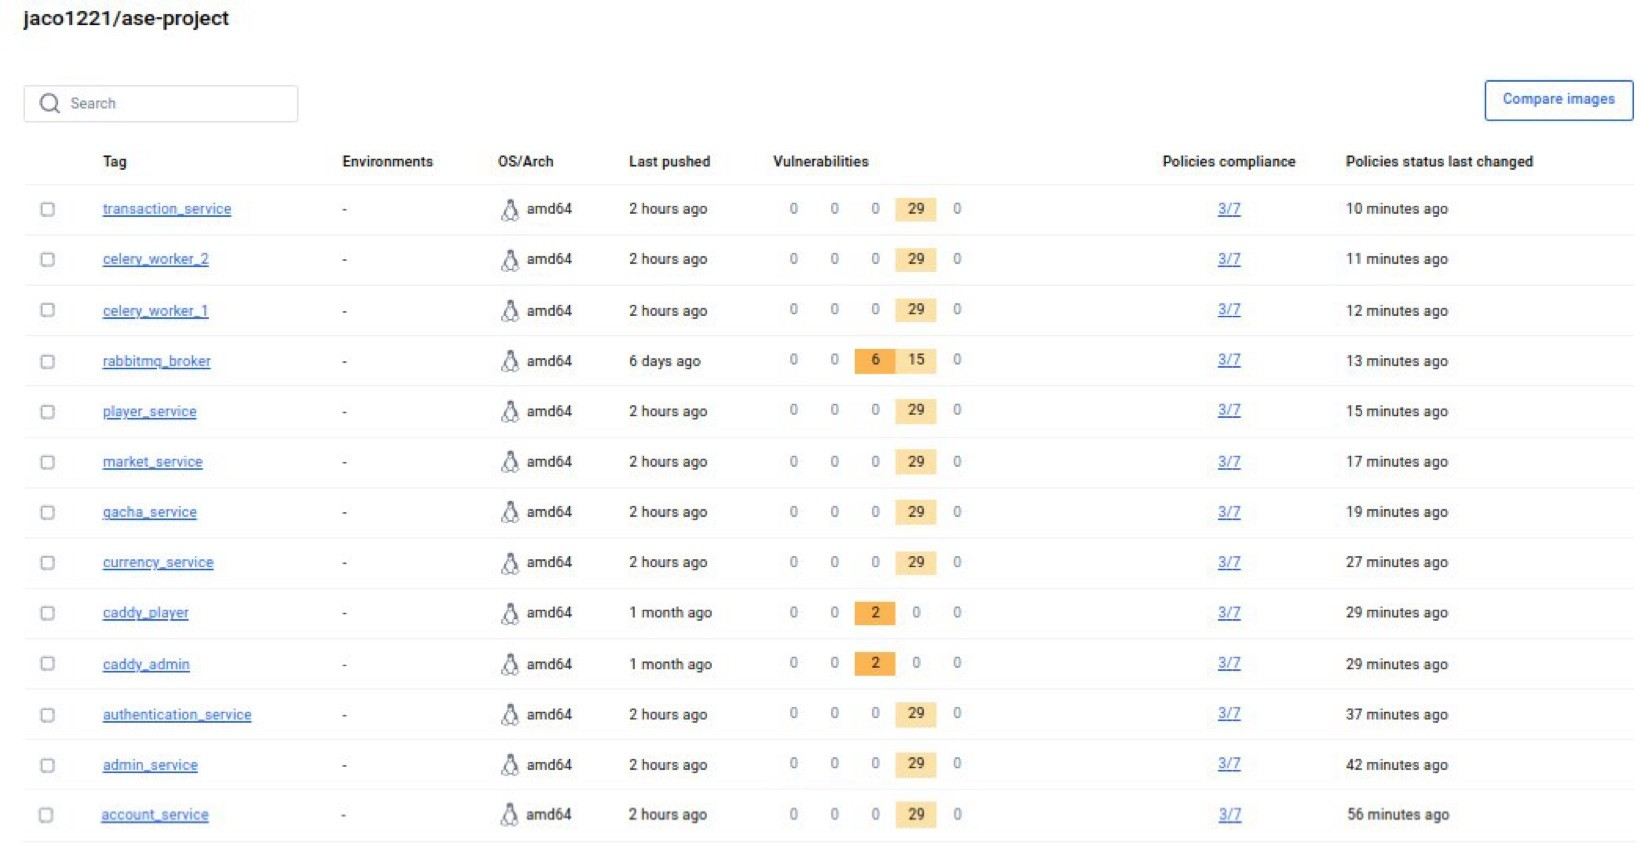
\includegraphics[width=\textwidth]{img/gacha/dashboardDockerScout.jpeg}
    \caption{Docker Scout dashboard with indicated vulnerabilities}
    \label{fig:docker_scout_dashboard}
\end{figure}

The developed Docker images are available in the following Docker Hub repository:
\href{https://hub.docker.com/r/jaco1221/ase-project/}{
https://hub.docker.com/r/jaco1221/ase-project/}
\newpage

\section{Additional features}
This section highlights features and considerations beyond the core functional requirements:

\subsection{Graphical User Interface}
\begin{itemize}
    \item \textbf{Purpose:} Enhance user experience and system accessibility.
    \item \textbf{Implementation:} Developed a web-based GUI using JavaScript and HTML.
    \item \textbf{Benefit:} Provides a more intuitive and user-friendly interaction with the gacha system.
\end{itemize}

\subsection{Additional Admin APIs}
\begin{itemize}
    \item \textbf{Auction Management APIs:}
        \begin{itemize}
            \item \textbf{Payment Forcing:} \texttt{'/admin/payment/<auction\_uuid>'}
            \item \textbf{Auction Closure:} \texttt{'/admin/close/<auction\_uuid>'}
            \item \textbf{Functionality:} Allows administrators to manually manage and resolve auction transactions.
        \end{itemize}

    \item \textbf{Player Transaction Oversight:}
        \begin{itemize}
            \item \textbf{Transaction Retrieval:} \texttt{'/admin/transaction/<user\_uuid>'}
            \item \textbf{Functionality:} Enables administrators to view complete transaction history for a specific player.
            \item \textbf{Purpose:} Facilitates administrative monitoring and potential fraud detection.
        \end{itemize}

    \item \textbf{Market Transparency:}
        \begin{itemize}
            \item \textbf{Closed Auction Visibility:} \texttt{'/admin/market'}
            \item \textbf{Functionality:} Allows administrators to view both open and closed auctions.
            \item \textbf{Purpose:} Provides comprehensive market oversight.
        \end{itemize}

    \item \textbf{User Management:}
        \begin{itemize}
            \item \textbf{User Deletion:} \texttt{'/admin/users/<user\_uuid>'}
            \item \textbf{Functionality:} Enables administrators to remove user accounts.
            \item \textbf{Purpose:} Provides administrative control over user base management.
        \end{itemize}
 We have furthermore validated the functionality of these implemented administrative APIs through the comprehensive testing methodologies detailed in Section \ref{sec:testing_approach}. These tests ensure the reliability, performance, and security of the newly introduced administrative endpoints.
\end{itemize}

\subsection{Authentication Token Management}
\begin{itemize}
    \item \textbf{Token Expiration Strategy:} In a real decentralized microservices architecture, the best solution is to maintaining a distributed token blacklist across services and implement a shared, synchronized mechanism to track and invalidate expired or logged-out tokens.
    \item \textbf{Current Implementation Limitations:}
        \begin{itemize}
            \item Logout mechanism currently relies on client-side JavaScript token removal.
            \item No server-side token invalidation during logout process.
        \end{itemize}
    \item \textbf{Recommended Improvements for Production:}
        \begin{itemize}
            \item Create a centralized or distributed token blacklist accessible by all microservices.
            \item Implement server-side token invalidation during logout.
            \item Enhance security by ensuring tokens are truly revoked across the entire system.
        \end{itemize}
    \item \textbf{Rationale:} The current JavaScript-based token removal is a simplified solution that does not provide comprehensive security in a distributed system.
\end{itemize}

\subsection{Docker Image Security Analysis}
\begin{itemize}
    \item \textbf{Scope:} Docker Scout vulnerability scanning did not cover third-party database image.
    \item \textbf{Specific Image:} \texttt{cybertecpostgresql/postgresql-ee-demo:16}.
    \item \textbf{Justification:} Image provides built-in SSL and encryption features managed by third-party vendor.
    \item \textbf{Recommendation:} Conduct additional security assessment for third-party images in future iterations.
\end{itemize}
\end{document}
